\chapter{Methodik}
In diesem Abschnitt wird die Vorgehensweise erläutert, mit der MRiLab auf Eignung als Simulationsumgebung untersucht wird, wie das MR-Signal mit Phasenrauschen gestört wird und wie Testsimulationen durchgeführt werden.

\section{MRiLab}
MRiLab wird auf einem PC mit einer High-End Consumer Grafikkarte installiert (siehe \autoref{sec:usedPC}). Aufwendige Rechnungen in MRiLab (wie das Lösen der Blochgleichungen für die einzelnen Voxel) sind gut parallelisierbar. Je nachdem, ob eine geeignete Grafikkarte für CUDA vorhanden ist, wird diese genutzt, oder die Berechnungen werden mit dem regulären Prozessor und IPP durchgeführt.

\autoref{fig:mrilabscreenshot} zeigt das Startfenster von MRiLab mit einem geladenen Gehirn-Phantom (mitgeliefert). Dieses wird über \texttt{Load>Phantom} ausgewählt und mit \texttt{Localize} in die mittleren drei Fenster geladen, welche die drei möglichen Schnittebenen durch einen Körper zeigen. Nach dem Einstellen grundlegender Parameter, wie der gewünschten Auflösung, können diese mit \texttt{Update} übernommen werden. Nach der Auswahl einer Pulssequenz über \texttt{Sequence}\footnote{Im Dialogfeld wird die Pulssequenz mit einem Doppelklick ausgewählt!} wird nach Betätigen von \texttt{Update} und \texttt{Scan} eine Simulation gestartet.

\begin{figure}[H]
	\centering
	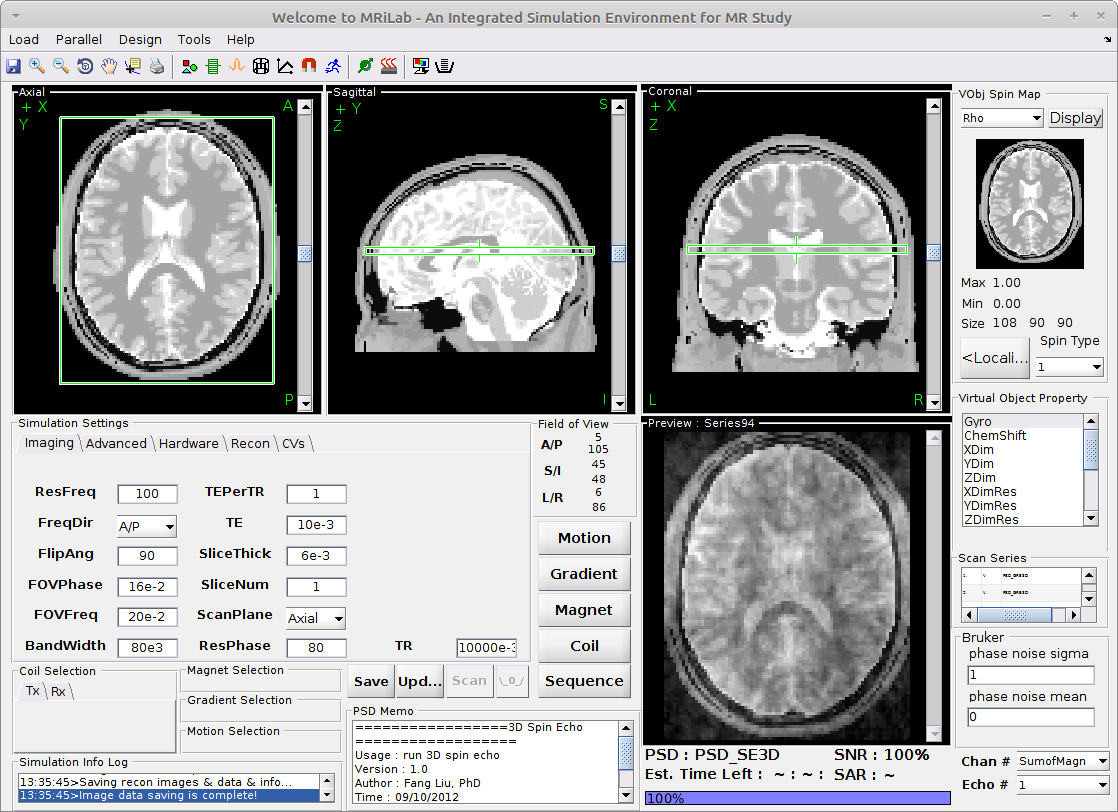
\includegraphics[width=\textwidth]{img/mrilabScreenshot.png}
	\caption[MRiLab Startbildschirm]{Startbildschirm von \textit{MRiLab} mit einem geladenen Gehirn Phantom und dem Simulationsergebnis einer Spinecho-Sequenz (unten rechts)}
	\label{fig:mrilabscreenshot}
\end{figure}

\subsection{Bestimmung notwendiger Simulationsparameter}
MRiLab verwendet einige Standardparameter für die MRT-Simulation, die sich an einem GE MRT für die Humanmedizin orientieren. Für diese Größen müssen die äquivalenten Werte für ein präklinisches MRT von Bruker gefunden werden. Die gesuchten Größen sind mit der in MRiLab verwendeten Terminologie in \autoref{tab:mriLabParam} aufgeführt.

In Abstimmung mit der Applikationsentwicklung für die MRT können einige Werte bzw. Wertebereiche, wie sie typisch für die aktuelle Produktpalette der Bruker MRTs sind, angegeben werden (siehe \autoref{tab:brukerMRIparam}). 

\begin{table}[H]
	\centering
	\caption[Bruker MRT Simulationsparameter]{Einige für die MRT Simulation in MRiLab relevante Parameter für Bruker MRTs}
	\label{tab:brukerMRIparam}
	\begin{tabularx}{\textwidth}{lX}
		\toprule
		\textbf{Parameter} & \textbf{Werte(-bereich)}\\
		\midrule
		FOVFreq    & typ. \SI{50}{\mm}, bis zu \SI{150}{\mm}\\
		FOVPhase   & typ. \SI{50}{\mm}, bis zu \SI{150}{\mm}\\
		ResFreq    & 128, 256 (64, 32 bei schnellen Sequenzen; 512, 1024, 2048 bei hochauflösenden Messungen)\\
		ResPhase   & etwa gleich wie ResFreq, tendenziell etwas weniger (z.B. $Res \times Freq=128\times256$)\\
		SliceThick & typ. \SI{0.5}{\mm}...\SI{1}{\mm} (min: \SI{0.2}{\mm}, max: einige wenige \SI{}{\mm})\\
		B0         & \SI{1}{\tesla}, \SI{3}{\tesla}, \SI{4.7}{\tesla}, \SI{7}{\tesla}, \SI{9.4}{\tesla}, \SI{11.7}{\tesla}, \SI{15.2}{\tesla} \\
		B1         & ca. \SI{10}{\micro\tesla}\\
		MaxGrad    & typ. \SI{200}{\milli\tesla\per\m}...\SI{1000}{\milli\tesla\per\m}\\
		MaxSlewRate& typ. \SI{500}{\tesla\per\m\per\s}...\SI{10000}{\tesla\per\m\per\s}\\
		\bottomrule
	\end{tabularx}
\end{table}

Die notwendige Bandbreite des Empfängers kann aus den bekannten Daten berechnet werden:

Unter der Annahme, dass der Probenraum quadratisch ist und die Gradientenstärken $G$ in $x$- und $y$-Richtung gleich sind, sind die Lamorfrequenzen an den Rändern des Probenraums in Frequenz- und Phasenkodierrichtung gleich:
\begin{subequations}
	\begin{align}
	f_{min}=\frac{\gamma}{2\pi} (B_0+G\; x_{min}) \\
	f_{max}=\frac{\gamma}{2\pi} (B_0+G\; x_{max})
	\end{align}
\end{subequations}
mit:
\begin{with}
	\frac{\gamma}{2\pi} =\SI{42.577478}{\mega\hertz\per\tesla}& Gyromagnetisches Verhältnis für \ce{^{1}H}-Kerne \\
	B_0 \text{~(in \SI{}{\tesla})} & Feldstärke statisches Magnetfeld \\
	G \text{~(in \SI{}{\tesla\per\meter})} & Gradientenstärke \\
\end{with}

Die notwendige Empfängerbandbreite $\Delta f$ ergibt sich daraus zu:
\begin{equation}
\Delta f = f_{max}-f_{min} = \frac{\gamma}{2\pi} G (x_{max}-x_{min})
\end{equation}
Da die Länge $x_{max}-x_{min}$ der Größe des $FOV$ in der betrachteten Richtung entspricht, kann $\Delta f$ berechnet werden mit:
\begin{equation}
\label{eq:deltaF}
\Delta f(G, FOV) = G \cdot FOV
\end{equation}

Mit Hilfe von \autoref{eq:deltaF} und typischen Werten für die Gradientenstärke und das FOV werden einige Empfängerbandbreiten berechnet (\autoref{tab:empfBandbreite}).

\begin{table}[H]
	\centering
	\caption[Berechnung Empfängerbandbreite]{Notwendige Empfängerbandbreiten in Abhängigkeit des Field of View (FOV) und der Gradientenstärke}
	\label{tab:empfBandbreite}
	\begin{tabular}{llll}
		\toprule
		& \multicolumn{3}{c}{\textbf{G (in \SI{}{\milli\tesla\per\meter})}} \\ \cmidrule{2-4}
		\textbf{FOV (in \SI{}{\mm})}& 200 & 500 & 1000 \\
		20 & \SI{0.170}{\mega\hertz} & \SI{0.425}{\mega\hertz} & \SI{0.851}{\mega\hertz} \\
		50 & \SI{0.426}{\mega\hertz} & \SI{1.06}{\mega\hertz} & \SI{2.13}{\mega\hertz} \\
		150 & \SI{1.277}{\mega\hertz} & \SI{3.19}{\mega\hertz} & \SI{6.39}{\mega\hertz} \\
		\bottomrule
	\end{tabular}
\end{table}

\section{Einfluss von Phasenrauschen auf das MR-Empfangssignal}
Aus der Erfahrung zeigt sich, dass Bildartefakte, wie sie durch Phasenrauschen des ADC-Taktsignals entstehen, sich stärker auf die subjektive Bildqualität auswirken, als zum Beispiel Amplitudenrauschen. Daher wird das MR-Empfangssignal mit verschiedenen Phasenrauschspektren beaufschlagt, um ein Phasenrauschen des ADC-Taktsignals nachzubilden.

Das Spektrum des Phasenrauschens eines realen Oszillators ist nicht konstant (weiß), sondern die spektrale Leistungsdichte strebt für sehr kleine Werte der Offsetfrequenz $f_{offset}=f-f_c$ gegen die des Trägers:
\begin{equation}
P(f_{offset} \rightarrow 0) = P_c
\end{equation}
Für große Frequenzen geht die Phasenrauschleistung gegen null. Es bleibt ein konstanter "noise floor" $N_0$:
\begin{equation}
	P(f_{offset} \rightarrow \infty) = N_0.
\end{equation}

\subsection{Generierung von Phasenrauschen}
Zur Simulation mehrerer Realisierungen $\xi_i$ des Phasenrauschprozesses $y_\xi(t)$ müssen Zufallszahlen verwendet werden. Fast alle Numerik-Pakete, so auch MATLAB, bieten eine Funktion zur Generierung von (pseudo) zufälligem weißen gaußschem Rauschen. "Weiß" bedeutet dabei, dass das Spektrum, in Anlehnung an die spektrale Bestrahlungsstärke einer weißen Lichtquelle, alle Frequenzen enthält. "Gauß" bedeutet, dass die Wahrscheinlichkeitsdichtefunktion der Funktionswerte eine Gaußkurve ist. Diese beiden Eigenschaften sind in \autoref{fig:randn} visualisiert.

\begin{figure}[H]
	\centering
	\subcaptionbox{Schätzung des Leistungsdichtespektrums mit einem Periodogramm }{\includegraphics[width=0.45\textwidth,height=0.35\textwidth]{plots/randnSpect.tikz}}
	\hfill
	\subcaptionbox{Schätzung der Wahrscheinlichkeitsdichtefunktion mit einem Histogramm}{\includegraphics[width=0.45\textwidth,height=0.363\textwidth]{plots/randnHist.tikz}}
	\caption[MATLAB randn]{Simulation von 1000 Zufallszahlen mit \texttt{X=randn(1,1000)} in MATLAB}
	\label{fig:randn}
\end{figure}

Zur Simulation von Phasenrauschen muss das Spektrum des weißen Gauß-Prozesses mit einem Formfilter verändert werden; es wird eingefärbt. Wie in \autoref{fig:faerben} gezeigt, kann diese Formung im Zeitbereich durch eine Faltung mit der Impulsantwort $g(t)$, oder im Frequenzbereich durch eine Multiplikation mit der Übertragungsfunktion $G(f)$ erfolgen

\begin{figure}[H]
	\centering
	\resizebox{14cm}{!}{\includegraphics[]{img/rauschSimu.tikz}}
	\caption[Erzeugen von farbigem Rauschen]{Erzeugung von farbigen Rauschen aus einem weißen Gaußprozess}
	\label{fig:faerben}
\end{figure}

Für beide grundsätzlichen Möglichkeiten gibt es mehrere Realisierungsmöglichkeiten. Die Umsetzung mit einem FIR- bzw. IIR-Filter und die punktweise Multiplikation der Spektren sind in den folgenden Abschnitten vorgestellt.

\subsubsection{Multiplikation im Frequenzbereich}
Die gemessenen bzw. durch ein Datenblatt erhaltenen Phasenrauschspektren sind gegenüber der nötigen Abtastwerte für eine Simulation $N\approx512^2$ nur durch vergleichsweise wenige Punkte $M\approx10...100$ gegeben. Für eine Filterung durch eine punktweise Multiplikation muss daher das Filterspektrum von $M$ auf $N$ interpoliert werden.

\subsubsection{Faltung im Zeitbereich (FIR/IIR Filter)}
Ist die Impulsantwort für einen geeigneten Formfilter gegeben, kann diese im Zeitbereich für eine Filterung verwendet werden. Zur Generierung der Übertragungsfunktion und damit der Impulsantwort können die Filterentwurfswerkzeuge von MATLAB verwendet werden.

\small{
\paragraph{Vorbemerkung:}\mbox{}\\
MATLAB verwendet in den Filterdesign-Tools der "Signal Processing Toolbox" normierte Frequenzen:
\begin{subequations}
	\begin{align}
	f_{norm} = \text{"normalized frequency"} &= \frac{2f}{f_S} \\
	\omega_{norm} = \text{"radian frequency"} &= \frac{2\pi f}{f_S}
	\end{align}
\end{subequations}
Für Frequenzen im sinnvollen Bereich $f\in [0,f_S/2]$ ergibt sich damit der Wertebereich von
$f_{norm}$ und $\omega_{norm}/\pi$ zu $\mathbb{W}_{f_{norm}}=\mathbb{W}_{\omega_{norm}/\pi}=[0,1]$.
}

Übliche (digitale) Filter, wie Tiefpässe, Hochpässe und Bandpässe/Bandsperren haben in der Regel einfach zu formulierende Designziele: Ein steiler Übergang von den Passbändern zu den Stoppbändern und eine jeweils kleine Welligkeit in den Bändern.
Für das Design solcher Filter bietet die \textit{Signal Processing Toolbox} in MATLAB einige Werkzeuge, wie z.B. den \textit{FilterDesigner} an.

Filter mit beliebigem Amplituden- bzw. Phasengang können damit nicht entworfen werden. Stattdessen eignet sich beispielsweise die Funktion \texttt{fir2()}, um die Filterkoeffizienten für einen FIR-Filter mit beliebigem Amplitudengang zu ermitteln\footnote{\texttt{cfirpm()} und \texttt{firpm()} sind weitere Möglichkeiten, einen FIR-Filter mit der "equiripple"- bzw. "Parks-McClellan"-Methode zu erzeugen.}. Ein IIR-Filter kann mit Hilfe der modifizierten Yule-Walker-Gleichungen und eines Least-Square-Fits durch die Funktion \texttt{yulewalk()} generiert werden.

\begin{figure}[H]
	\centering
	\subcaptionbox{FIR-Filter, Ordnung $n=1000$}{\includegraphics[width=0.45\textwidth,height=0.5\textwidth]{plots/fir.tikz}}
	\hfill
	\subcaptionbox{IIR-Filter, Ordnung $n=70$}{\includegraphics[width=0.45\textwidth,height=0.5\textwidth]{plots/iir.tikz}}
	\caption{Näherung eines Spektrums durch zwei digitale Filter}
	\label{firIirPhasenoise}
\end{figure}

\subsection{Interpretation des Phasenrauschens als Zeitverschiebung}
Das Hinzufügen von Phasenrauschen zu einem abgetasteten Signal kann als eine Verschiebung der Abtastzeitpunkte aufgefasst werden. \autoref{fig:abtast} zeigt eine Funktion $x(t)$ und die abgetastete Funktion $x[n]$, die an den Stellen $n_0,\,n_1,\,\dots$ definiert ist. Jeder Abtastzeitpunkt wird um $\Delta t\,n$ verschoben. Die Wahrscheinlichkeitsdichtefunktion von jedem $Delta t,\,n$ ist dabei $f_{Delta t,\,n}$. In \autoref{fig:abtast} ist für jeden Abtastzeitpunkt $n$ eine Gauß-förmige Wahrscheinlichkeitsdichte gewählt. Mit dieser Methode können sinnvoll nur kurzzeitige Abweichungen simuliert werden. Zur Charakterisierung würden sich der edge-to-edge-Jitter oder der k-cycle-Jitter (für kleine $k$) eignen.

\begin{figure}[H]
	\centering
	\resizebox{!}{!}{\includegraphics[width=0.5\textwidth]{img/abtast.tikz}}
	\caption[Verschiebung der ADC Abtastzeitpunkte]{Verschiebung der ADC Abtastzeitpunkte mit einer Gauß-förmigen Wahrscheinlichkeitsverteilung für jeden Abtastzeitpunkt}
	\label{fig:abtast}
\end{figure}

Zur Untersuchung der Einflüsse von größeren Abweichungen, wie sie insbesondere durch die Akkumulation von Phasenfehlern entstehen können, ist diese Vorgehensweise nicht ideal.

Eine Zeitverschiebung um $\Delta t$ entspricht, mit der Frequenz der Grundschwingung $\nu_0$, einer Phasendrehung von
\begin{equation}
	\Delta \phi = 2 \pi \Delta t.
\end{equation}

Die Verschiebung der Abtastzeitpunkte lässt sich dann durch
\begin{equation}
	x_{Jitter}[n] = x[n] \quad exp(j \Delta \phi)
\end{equation}
beschreiben. Vorteil hierbei ist, dass neben Kurzzeit- auch Langzeit-Jitter problemlos simuliert werden kann.

Zur Demonstration der Äquivalenz der beiden Verfahren wird ein Sinus-Signal $S[n]=S_x+j S_y$ der Länge $N$ betrachtet. Weiterhin wird ein Tiefpass-gefilterter Phasenrauschprozess $\Delta t$ bzw. $\Delta \phi$ erzeugt. Dieser besitzt eine Gauß-förmige Wahrscheinlichkeitsdichtefunktion und einen $1/f$-förmiges Spektrum.

$S[n]$ wird zunächst zu $S[m]$ mit $M \gg N$ interpoliert. Danach können die ursprünglichen Abtastpunkte $n$ mit einem leichten Jitter ($\Delta t$) verschoben werden. Daraus entsteht $S[n_{Jitter}]$. Wird $S[n_{Jitter}]$ an den Stellen $n$ ausgewertet, entsteht $S_{Jitter}[n]$.

Wenn die Originalfunktion $S[n]=S_x+j S_y$ mit $exp(j \Delta \phi)$ multipliziert wird, entsteht $S_{PhaseMod}[n]$. Wie \autoref{fig:abtastPlot} bestätigt, liefern beide Vorgehensweisen ähnliche Resultate. Durch die nötigen, mehrfachen Interpolationen und Dezimierungen sind die Ergebnisse nicht identisch. 

\begin{figure}[H]
	\centering
	\resizebox{!}{!}{\includegraphics[width=1\textwidth,height=0.4\textwidth]{plots/abtastPlot.tikz}}
	\caption[Verschiebung Abtastzeitpunkte]{Verschiebung der Abtastzeitpunkte im Vergleich zur Originalfunktion; dargestellt sind jeweils die Realteile der Funktionen}
	\label{fig:abtastPlot}
\end{figure}

\subsection{Phasenrauschfunktion für MRiLab}
Das erzeugte Phasenrauschen kann nun auf das, digital vorhandene, komplexe MR-Empfangssignal $S_{RF}[n]$ gegeben werden. In MRiLab werden statt $S_{RF}[n]$ die beiden Signale \texttt{VSig.Sx} und \texttt{VSig.Sy} verwendet. Daher wird die Operation in \autoref{lst:vsigAddphaseNoise} durchgeführt.
\begin{listing}[H]
	\begin{minted}[bgcolor=bg,fontsize=\footnotesize,linenos,autogobble]
	{Matlab}
	S_rf = VSig.Sx + 1j*VSig.Sy;
	S_rf = S_rf .* exp(-1j*phaseNoise)
	VSig.Sx = real(S_rf);
	VSig.Sy = imag(S_rf);
	\end{minted}
	\caption{Anwendung von Phasenrauschen auf das MR-Empfangssignal}
	\label{lst:vsigAddphaseNoise}
	\end{listing}
	


\subsection{Gewinnung verschiedener Leistungsspektren}

\subsubsection{LMK04821 unter Idealbedingungen}
Im Datenblatt des Jitter-Cleaner Bausteins für Taktsignale \textit{LMK04821} von Texas Instruments \cite{lmkDatasheet} finden sich für verschiedene Betriebszustände gemessene Phasenrauschspektren. Dadurch, dass die Spektren als Screenshots des verwendeten Messgerätes abgebildet sind, ist zu erkennen, dass zur Messung ein Agilent Technologies (heute Keysight Technologies) \textit{E5052A Signal Source Analyzer} verwendet wurde. Dadurch, dass bei den Messungen die Option zur automatischen Konversion vom Phasenrauschspektrum zu Jitter genutzt wurde, können die Screenshots zur Validierung eigener Rechnungen verwendet werden. 

In \autoref{fig:lmkDatasheetPhaseNoise} ist das Phasenrauschspektrum des LMK04821 für einen möglichen Betriebszustand dargestellt. In der Abbildung sind die Einzelwerte der tabellarischen Aufführung des Spektrums entnommen. Da der Baustein in diesem Fall unter idealen Laborbedingungen betrieben wurde, ergibt dieses Phasenrauschspektrum eine untere Abschätzung.

\begin{figure}[H]
	\centering
	\resizebox{!}{!}{\includegraphics[width=1\textwidth,height=0.4\textwidth]{plots/lmkDatasheet.tikz}}
	\caption[LMK08421 Phasenrauschspektrum]{LMK04821 Phasenrauschspektrum \cite[S.~24, Figure 2]{lmkDatasheet}}
	\label{fig:lmkDatasheetPhaseNoise}
\end{figure}


\subsubsection{LMK04821 Realbedingungen und Worst-Case Abschätzung}
Für eine Worst-Case Abschätzung wird ein LMK04821-Testboard\footnote{LMK04828BEVM \cite{lmkEvalboard}} im Inneren eines BioSpec MR-Tomographen platziert. Bedingt durch die Größe des Testboards kann es nicht in die Hochfrequenz Sende- und Empfangsspulen-Röhre geschoben werden. Daher wird diese im Gerät nach hinten verschoben, so dass das Testboard in die Öffnung des Gradientensystems passt (siehe \autoref{fig:lmkinBioSpecRender}). Mit Hilfe eines Keysight Technologies \textit{N9952A} Spektrumanalysators wird das Spektrum am Ausgang des LMK04821 gemessen. Der verwendete Tomograph nutzt eine supraleitende Spule zur Erzeugung des $B_0$-Feldes, wodurch dieses nicht ohne weiteres abgeschaltet werden kann. Es ist daher während allen Versuchen aktiv.

\begin{figure}[H]
	\centering
	\resizebox{!}{!}{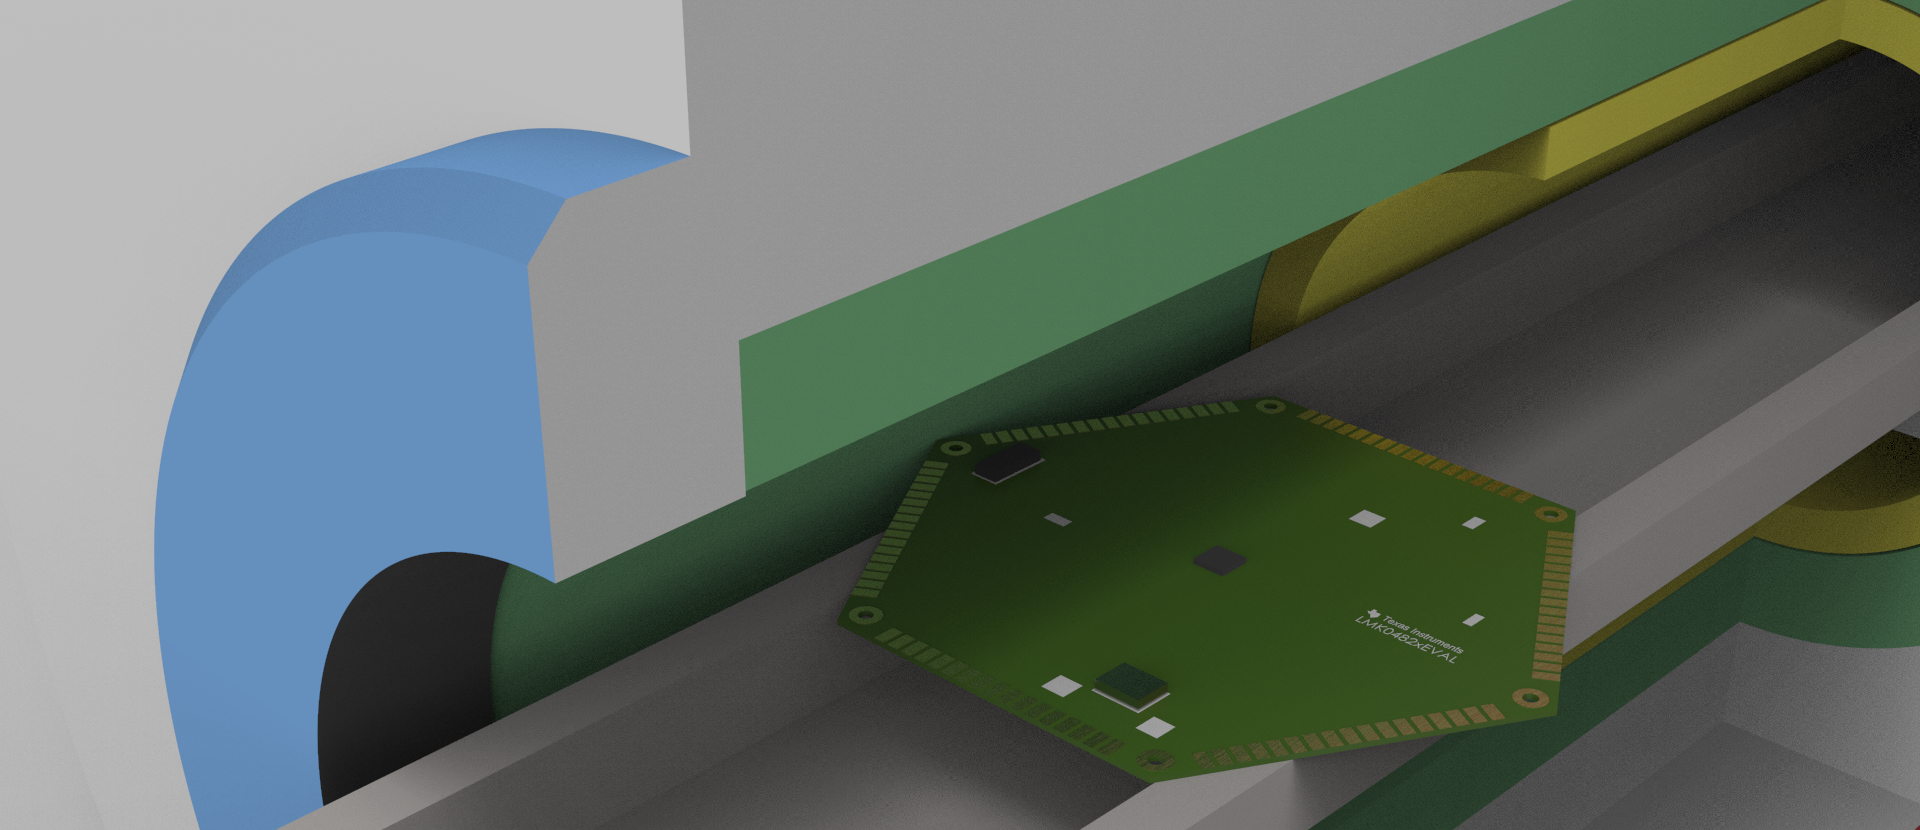
\includegraphics[width=0.6\textwidth]{img/lmkInBiospecCrop.png}}
	\caption[LMK04821 Position in Tomograph]{Positionierung des LMK04828BEVM im MR-Tomograph (Schnittbild); blau: vordere Öffnung; grün: Gradientensystem; gelb: Sende- und Empfangsspulen (ins Gerät hinein geschoben)}
	\label{fig:lmkinBioSpecRender}
\end{figure}

Zunächst wird der Einfluss des $B_0$-Feld untersucht. Dazu wird das Leistungsspektrum für eine Positionierung vor der MRT Öffnung und in der MRT Bohrung (wie in \autoref{fig:lmkinBioSpecRender} gezeigt) aufgenommen. Der Vergleich der beiden Spektren in \autoref{fig:lmkEttlingenBioSpecB0} zeigt, dass das $B_0$-Feld allein keine nachweisbaren Auswirkungen auf das Phasenrauschen hat.

\begin{figure}[H]
	\centering
	\resizebox{!}{!}{\includegraphics[width=1\textwidth,height=0.4\textwidth]{plots/lmkBioSpecNurB0.tikz}}
	\caption[]{Ausgangsspektrum des LMK04821 beim Betrieb in der Nähe des MRT und im MRT (ohne aktives Gradientensystem und ohne RF-Signale); Betrieb des Spektrumanalysators mit "Maximum Hold"}
	\label{fig:lmkEttlingenBioSpecB0}
\end{figure}

Für die Nachbildung einer realen MRT Messung wird eine RARE MRT-Pulssequenz abgefahren. Dabei werden die Gradientenfelder mit der Repetitionszeit $TR$ geschaltet. Für zwei verschiedene Repetitionszeiten sind die Spektren in \autoref{fig:lmkEttlingenBioSpecGradients} dargestellt. Es sind dabei jeweils zwei Spektren mit unterschiedlichen Aufnahme-Modi des Spektrumanalysators gezeigt:
\begin{itemize}
	\item \textbf{Maximum Hold:} Bildet das Maximum über mehrere aufgenommene Spektren. Geeignet zum Festhalten kurzzeitig präsenter Anteile im Spektrum.
	\item \textbf{Trace Averageing:} Bildet den Mittelwert über mehrere aufgenommene Spektren. Kurzzeitige Fluktuationen werden entfernt.
\end{itemize}

\begin{figure}[H]
	\centering
	\subcaptionbox{$TR=\SI{2.4}{\milli\second}$}{\includegraphics[width=1\textwidth,height=0.4\textwidth]{plots/lmkBioSpecG1.tikz}}
	\\[4ex]
	\subcaptionbox{$TR=\SI{1.5}{\milli\second}$}{\includegraphics[width=1\textwidth,height=0.4\textwidth]{plots/lmkBioSpecG2.tikz}}
	\caption{LMK04821 Betrieb in BioSpec MR-Tomograph bei aktiver Pulssequenz}
	\label{fig:lmkEttlingenBioSpecGradients}
\end{figure}

\subsection{Umrechung in Phasenrauschleistungsspektren}



\section{Erstellung MRT Phantom}
Für die Simulationen mit MRiLab sind Eingangsobjekte nötig. Diese können zum Beispiel reale MRT-Aufnahmen von Lebewesen oder Prüfkörpern (genannt Phantome) sein, oder rein digital erzeugt sein. Da es für die Zukunft wünschenswert ist, Simulationsergebnisse mit realen Messungen zu verifizieren, bietet sich die Nutzung einer digitalen Abbildung eines real existierenden Phantoms an.

Für die kontinuierliche Qualitätsüberwachung in Kliniken und radiologischen Praxen bieten Händler für MRT-Zubehör verschiedene MRT-Phantome an. Diese bestehen meist aus flüssigkeitsgefüllten Kunststoffstrukturen, häufig PMMA. Im Inneren verfügen diese Phantome über verschiedene Einsätze, um bestimmte Eigenschaften eines MR-Tomographens zu bewerten. So lässt sich beispielsweise über ein regelmäßiges Gitter eine Aussage über geometrische Verzerrungen und durch eine Keilplatte eine Aussage über die Schichtdicke machen. Durch abgedichtete Einsätze können Flüssigkeiten mit abweichenden NMR-Eigenschaften als die Hauptflüssigkeit eingebracht werden. Eine Auswahl von kommerziell erhältlichen Phantomen ist in \autoref{tab:phantomsOverview} zusammengestellt.

Aufgrund des kleineren freien Innendurchmessers präklinischer MRTs sind diese Phantome jedoch entweder deutlich zu groß, oder bieten ein schlechtes Preis/Leistungsverhältnis. In der Vergangenheit wurde daher von der internen Konstruktionsabteilung bei Bruker BioSpin ein Phantom mit \SI{63}{\mm} Außendurchmesser entwickelt und von der Mechanikwerkstatt am Standort Rheinstetten gefertigt (siehe \autoref{fig:63mmPhantom}). Es besteht aus mehreren PMMA-Kunststoffelementen in einem PMMA-Hohlzylinder. Das große Hohlvolumen des Zylinders und die Hohlvolumina der kleinen Hohlzylinder-Einsätze können unabhängig voneinander mit Flüssigkeiten gefüllt werden. Meist werden verschieden stark konzentrierte Salzlösungen verwendet, deren NMR-Eigenschaften bekannt sind. Dadurch bietet dieses Phantom alle nötigen Merkmale und wird deshalb im weiteren Verlauf dieser Arbeit verwendet.

 Da der Fertigungsaufwand für einen solchen Kunststoffkörper aus mehr als 20 Einzelteilen sehr hoch ist, lohnt sich die Auslieferung solcher Phantome zum Kunden der MR-Tomographen nicht. Für eine Demonstration der Gerätefunktionalitäten nach der Montage vor Ort und für die Evaluierung grundlegender Qualitätsanforderungen an den Tomograph wird das "50ml-Phantom" (siehe \autoref{fig:50mlPhantom}) eingesetzt. Es besteht aus einem \SI{50}{\milli\liter} Zentrifugenröhrchen (vgl. Datenblatt des Herstellers in \cite{corningCentriStar}) gefüllt mit einem Kupfer(II)-sulfat enthaltenden Gel. Darin eingebettet ist ein 2x4-LEGO Stein aus ABS. Durch die engen Fertigungstoleranzen, bekannten Maße und den günstigen Preis eignen sich LEGO-Steine gut als Referenzelemente.

\begin{figure}[H]
	\centering
	\subcaptionbox{"50ml-Phantom" (SNR und Auflösung)\label{fig:50mlPhantom}}{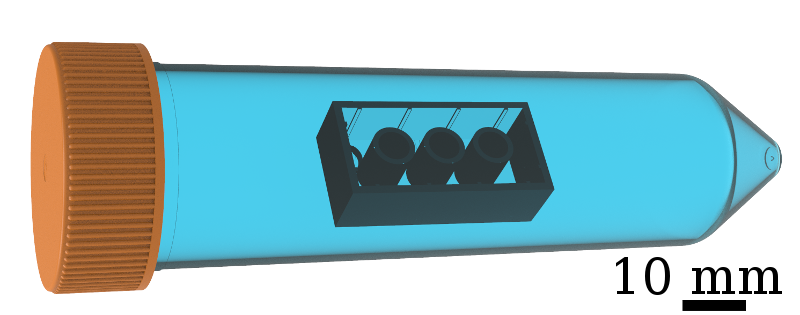
\includegraphics[width=0.45\textwidth]{img/phantoms/legoPhantom_scale.png}}
	\hfill
	\subcaptionbox{"63mm-Phantom" (Auflösung, Schichtdicke, SNR)\label{fig:63mmPhantom}}{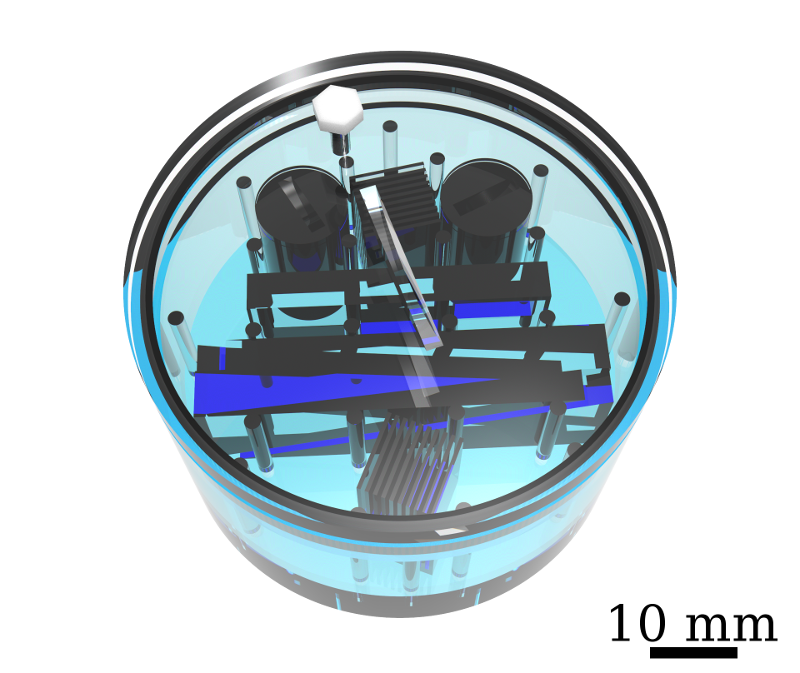
\includegraphics[width=0.45\textwidth]{img/phantoms/bkr60_scale.png}}
	\caption{Zwei bei Bruker BioSpin MRI eingesetzte MRT Phantome (Rendering)}
\end{figure}

Das Bruker 63mm-Phantom liegt zunächst nur in Form einer 2D Baugruppenzeichnung und der dazugehörigen (2D\footnote{Dateiformat: AutoCAD .dwg}) Einzelteilzeichnungen vor. Die nötigen Schritte, um daraus eine MRiLab \texttt{VObj*.mat} Phantom-Datei zu erzeugen, sind nachfolgend aufgezeigt.

\subsection{Erstellung eines 3D-CAD Modells}
Zunächst werden aus den zweidimensionalen Einzelteilzeichnungen 3D-Modelle erstellt. Da (mechanische) CAD-Modelle und Baugruppen verschiedener Softwarepakete in der Regel nicht kompatibel sind, werden die Modelle mit dem bei Bruker BioSpin verwendeten \textit{Siemens PLM Solid Edge} erstellt, um eine spätere Wiederverwendung in der Abteilung zu ermöglichen. Die Einzelteile werden anschließend, basierend auf der 2D-Übersichtszeichnung, zu einer Baugruppe zusammengesetzt. Das dabei entstehende Phantom-Modell ist noch luftgefüllt. Da in einer realen Messung die größten MR-Signale aus der Flüssigkeitsfüllung resultieren, kann die Füllung für die Simulation nicht vernachlässigt werden. Da Solid Edge keinen Assistent zur Füllung von Hohlräumen anbietet, muss die Füllung zunächst durch einen Vollzylinder angenähert werden. Von diesem werden dann durch eine Bool'sche Operation die inneren PMMA-Strukturen und die Flüssigkeiten der kleinen Hohlzylinder abgezogen. Es zeigt sich, dass in Solid Edge ST10 nicht gelingt eine Subtraktion von mehr als etwa sechs Einzelteilen durchzuführen.

Zur Lösung dieses Problems wird die Baugruppe mit allen Einzelteilen in \textit{SolidWorks 2014} (von der Dassault Systèmes SolidWorks Corp.) importiert. Da beim Import lediglich die Geometrien geladen werden und die einzelnen Features verloren gehen, wird der "Recognize Features"-Assistent eingesetzt, um aus dem importieren Körpern wieder ein vollständiges CAD-Modell zu erhalten. Vor Anwenden der Subtraktionsoperation auf den Flüssigkeitskörper müssen am Modell kleinere Änderungen vorgenommen werden, um sog. "zero-thickness geometries"\footnote{Die deutsche Bezeichnung "Geometrie der Dicke Null" ist nicht gebräuchlich} zu vermeiden. Zero thickness (auch  "non-manifold") Geometrien entstehen, wenn Kanten oder Eckpunkte einer Geometrie nicht richtig mit angrenzenden Geometrien verbunden werden können. Per Definition muss jede Kante genau zwei angrenzende Flächen haben. Wird diese Bedingung verletzt, kann es zu Problemen mit der Repräsentation der 3D-Geometrie im Modellierungskern der CAD-Software kommen.

\begin{figure}[H]
	\centering
	\resizebox{!}{!}{\includegraphics[width=0.33\textwidth]{img/zeroThickness.tikz}}
	\caption[Zero Thickness]{Zwei Möglichkeiten für die Entstehung von "zero thickness geometries": An den markierten Punkten hätte eine Kante, die in die Zeichenebene hineinläuft, mehr als zwei benachbarte Flächen ((1): 4 Kanten, (2): 3 Kanten)}
	\label{fig:zeroThick}
\end{figure}

Für die Positionierung der geraden Einsätze im Phantom relativ zu den dünnen Stäben kann daher keine Tangential-Beziehung verwendet werden. Durch Einfügen eines kleinen Abstandes wird die Entstehung von zero thickness geometry vermieden.

Nach der Behebung der zero thickness Probleme können alle Einsätze vom Flüssigkeitszylinder subtrahiert werden. Die Einzelteile und die Baugruppe werden im proprietären SolidWorks Format .SLDPRT bzw. .SLDASM und zusätzlich in den herstellerneutralen CAD-Austauschformat .IGES und .STEP abgespeichert.

\subsection{Konvertierung in eine 3D-Voxel-Matrix}
Die CAD-Dateiformate IGES und STEP enthalten jeweils eine Beschreibung der CAD-Daten in Form von Geometrieprimitiven und Features. Damit ist ein verlustfreier Ex- und Import zwischen verschiedenen Anwendungen möglich. Für die Konvertierung in eine Voxeldarstellung sind diese Formate jedoch ungeeignet, weil die Geometrien vor einer Rasterung zunächst aus der analytischen Darstellung in eine numerische gebracht werden müssen. Eine Möglichkeit ist der Export in eine .STL Datei. In (ASCII) STL Dateien wird eine Geometrie durch eine Vielzahl von, im Raum orientierter, Dreiecke angenähert (siehe \autoref{lst:STLspec}).

Eine Speicherung in STL ist daher in der Regel verlustbehaftet. Neben der genauen Geometriebeschreibung gehen beim Export aus SolidWorks in STL alle Informationen zu Features, Material etc. verloren. Daher wird das Phantom nicht als komplette Baugruppe exportiert, sondern es wird jedes Einzelteil separat exportiert. Um die Einzelteile in der STL Darstellung gegeneinander ausrichten zu können und Skalierungsproblemen beim Voxelisierungsprozess zu vermeiden, wird eine, das gesamte Phantom umspannende Referenzgeometrie eingeführt. Diese kann später ausgeblendet werden.

Die STL Dateien der Einzelteile müssen nun in eine Voxeldarstellung gebracht werden. Dazu wird das Python Skript \textit{stl-to-voxel} \cite{stlToVox} verwendet. Beim Versuch, eine mit SolidWorks exportierte STL zu verarbeiten, bricht das Skript jedoch mit einer Fehlermeldung ab. Die Fehlerursache und eine mögliche Fehlerbehebung sind in \autoref{sec:stlToVoxFix} beschrieben.

Stl-to-voxel kann nun eingesetzt werden, um \textbf{eine} STL Datei in einen Stack aus png Bildern zu zerlegen, die dann gestapelt die gesuchte Voxeldarstellung ergeben.
Der Aufruf von stl-to-voxel erfolgt beispielsweise mit:
\begin{listing}[H]
	\begin{minted}[bgcolor=white,fontsize=\footnotesize,autogobble,escapeinside=||]
	{bash}
	python3 ./stltovoxel.py ./inputSTLs/stlFile.stl ./outputFolder/filename.png 256
	\end{minted}
\end{listing}

Im Beispiel entspricht die 256 der gewünschten Auflösung $N$ des png-Stacks. Da nur eine Auflösung angegeben werden kann, entstehen immer $N$ $(N\times N)$ große png Bilder. Die png-Bilder haben eine Samplingtiefe/Bittiefe von $1$-Bit. Daher gilt für jeden Pixelwert:
\begin{equation}
	I = I(x,y) , \quad I(x,y) \in \{0, 255\}
\end{equation}
Ein Stapel aus unkomprimierten 1-Bit-Bitmaps hätte damit die Größe
\begin{equation}
	L=\SI{1}{\Bit} \cdot (N \times N) N = N^3 \,\SI{}{\Bit} = \frac{N^3}{8} \SI{}{\Byte}.
\end{equation}
Mit $N=256$ ergibt sich $L\approx \SI{2}{\mega\Byte}$ und mit $N=512$ ergibt sich eine Größe von $L\approx \SI{17}{\mega\Byte}$. Da png eine Komprimierung benutzt, sind die Berechnungen mit unkomprimierten Bitmaps eine obere Abschätzung\footnote{Erste Versuche ergeben für $N=512$ eine Größe von $L<\SI{300}{\kilo\Byte}$}.

Der Vorgang wird für alle $M$ Einzelteile wiederholt.

\subsection{Zusammenführen in eine .mat-Datei}
Die Voxelrepräsentation des Phantoms besteht jetzt aus $M$ Ordnern für jedes Einzelteil, die jeweils $N$ $(N \times N)$ große png Bilder enthalten. Diese müssen nun zu einer MATLAB Matrix kombiniert werden.

Zunächst werden die png Stacks jedes Einzelteils zu einer Matrix zusammengesetzt. Dazu werden die Bilder sequenziell in eine 2D-Matrix eingelesen. Die 2D-Matrizen werden dann aneinander gefügt, bis eine quadratische 3D-Matrix entstanden ist. Diese Einzelteilmatrizen werden dann in einer Matrix vereint.

Die Kombination der Einzelteile in einer Matrix kann zum Beispiel über eine Addition (der jeweils gleich großen Einzelmatrizen) erfolgen. Eine solche Operation wäre im Allgemeinen nicht umkehrbar. Da es sich aber bei den Einzelteilmatrizen um disjunkte Mengen handelt, können sie problemlos addiert werden.

Da Gewebe nicht nur eine, für die MRT relevante, Eigenschaft aufweist, ist eine Matrix zur vollständigen Beschreibung nicht ausreichend. MRiLab verwendet daher vier Eigenschafts-Matrizen $A_e$: Je eine für die Protonendichte (PD) und die Relaxationszeiten (T1, T2 und T2*).

Vor der Addition der Einzelteile zu einer dieser Matrizen wird daher jedes Einzelteil mit einer, für sein Material charakteristischen Konstante skaliert. Die Skalierungsfaktoren werden in Textdateien zusammen mit den png-Stacks in den Einzelteilordnern abgespeichert. Damit ergibt sich für eine Eigenschaftsmatrix:
\begin{equation}
\label{eq:sumMatrix}
	A_e=\sum_{i=1}^{M} k_{i,e} \underbrace{\sum_{n=0}^{N} I_n(x,y)}_\text{Einzelteilmatrix}
\end{equation}
mit:
\begin{with*}
	A_E & Matrix der Eigenschaft $e$, mit $e \in \{PD,\, T1,\, T2,\, T2\text{*}\}$ \\
	M & Anzahl der Einzelteile \\
	N & Auflösung der png Bilder und Anzahl der png Bilder \\
	I_n(x,y) & n-tes png Bild \\
\end{with*}

Der durch \autoref{eq:sumMatrix} beschriebene Algorithmus ist als MATLAB Skript in \autoref{lst:combinePhantomStacksIntoVoxelMatrix} zu finden.











